\documentclass{article}
\usepackage{pgfplots}
\pgfplotsset{compat=newest}

\pagestyle{empty}

\begin{document}

\begin{titlepage}
   \vspace*{\stretch{1.0}}
   \begin{center}
      \Large\textbf{Empirical Analysis of Sum of Maximum Subarray}\\
      \large\textit{Roland Shum, CS330}
   \end{center}
   \vspace*{\stretch{2.0}}
\end{titlepage}

\section{Problem statement}

The {\it maximum subarray} of a given sequence
is the contiguous subarray within a one-dimensional array of numbers which has the largest sum.
The task is to find the maximum subarray within a one-dimensional array. This is solved by using
Kadane's algorithm. This is already a solved issue. \newline

A far more interesting question is -- given a randomly generated sequence of a given length what is 
the average number the maximum subarray sums to? \newline

That is, given a randomly generated one-dimensional array of a given length, we want to find the function that relates 
the maximum subarray sum to the length of the array.

\section{Experiment setup}
To generate a sequence of length $N$ each element is independently generated
using uniform distribution of integers in the range $[0, {\it max int number}]$ using a Mersenne Twister algorithm.
For each $N$ we performed $200$ experiments, solving the Maximum Subarray Sum using Kadane's algorithm. 
The blue graph below shows the average value of the longest increasing subsequence plus-minus standard deviation.
The red graph shows function $f(x) = \frac{x^2}{2}$ which grows almost at the same rate, supporting 
the hypothesis that average sum of maximum subarray of size $N$
is $O($N$^2)$.


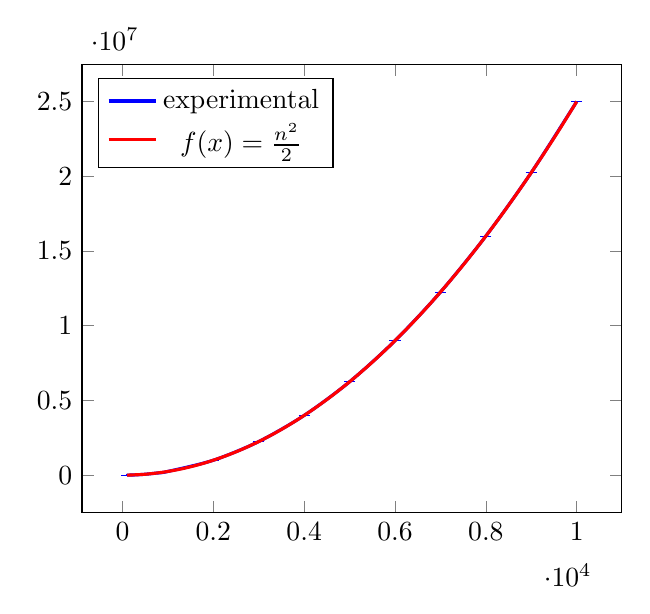
\begin{tikzpicture}
\begin{axis}[legend pos=north west]
\addplot+[line width=0.4mm,smooth,mark=,error bars/.cd, y dir=both,y explicit ]
    coordinates {
    (100, 2487.05) +- (22.3653191347675,22.3653191347675)
    (200, 9980.45) +- (45.6734879333734,45.6734879333734)
    (300, 22467.375) +- (72.3140676148148,72.3140676148148)
    (400, 39950.59) +- (90.1288072704837,90.1288072704837)
    (500, 62437.185) +- (116.089968451197,116.089968451197)
    (750, 140917.44) +- (165.597966171086,165.597966171086)
    (1000, 249914.535) +- (225.910178555549,225.910178555549)
    (2000, 999746.955) +- (480.686460153602,480.686460153602)
    (3000, 2249659.26) +- (724.929543059185,724.929543059185)
    (4000, 3999479.825) +- (983.678338876586,983.678338876586)
    (5000, 6249303.08) +- (1182.61043611157,1182.61043611157)
    (6000, 8999323.515) +- (1435.22032098734,1435.22032098734)
    (7000, 12249341.38) +- (1857.47349526178,1857.47349526178)
    (8000, 15998974.255) +- (1811.96749142334,1811.96749142334)
    (9000, 20248839.015) +- (2147.59163128724,2147.59163128724)
    (10000, 24998615.29) +- (2192.51952691418,2192.51952691418)
    };
\addlegendentryexpanded{experimental}
\addplot+[line width=0.4mm,smooth,mark=,domain=100:10000] {(x/2)^2};
\addlegendentryexpanded{$f(x) = \frac{{n}^2}{2}$}
\end{axis}
\end{tikzpicture}
\newline
\newline
Roland Shum
\end{document}
